\documentclass[12pt]{article}
\usepackage{amsmath,amssymb,amsthm}
\usepackage{graphicx,mathabx}
\usepackage{xcolor}
\usepackage{tikz}
\usepackage{placeins}
\usepackage{lipsum}
\usepackage[shortlabels]{enumitem}
\usepackage{placeins}
\usepackage[makeroom]{cancel}
\usepackage{mathrsfs}
\usepackage{nicefrac}
\newcommand\tab[1][1cm]{\hspace*{#1}}
\def\blankpage{%
      \clearpage%
      \thispagestyle{empty}%
      \addtocounter{page}{-1}%pdf
      \null%
      \clearpage}
\begin{document}
\title{TCSS 343 - Week 8}
\author{Jake McKenzie}
\maketitle
\noindent\centerline{\textbf{Graph Algorithms}}\\\\\\\\\\\\
\begin{center}
    ``If you've never missed a flight, you’re spending too much time in airports." \\$\dots$\\ Umesh Vazirani
\end{center}
\begin{center}
    ``Programming has things called ``threads" and things called ``strings" and they somehow have **** all to do with each other." \\$\dots$\\ Ramsey Nasser
\end{center}
\begin{center}
    ``Nothing in life is to be feared, it is only to be understood. Now is the time to understand more, 
    so that we may fear less." \\$\dots$\\ Marie Curie
\end{center}
\newpage
\noindent So when I was taking TCSS 343 I identified two core ideas of Dijkstra's algorithm. 
I'm going to present them to you for you to think about, then ask you to complete the algorithm.\\\\
\textit{How does Dijkstra's algorithm find new paths and do the}\textbf{ relaxation step}\textit{?}\\\\
\textit{In which order does Dijkstra's algorithm} \textbf{process }\textit{the vertices one by one?}\\\\
0. Fill in the rest of the algorithm for relaxing an individual edge.\\
Relax(u,v) $\{$\\
    $\tab$ if ( $\_\_\_\_\_\_\_\_\_\_\_\_\_\_\_$ $<$ d[v]) \{\\
        $\tab\tab\_\_\_\_\_\_\_\_\_\_\_\_\_\_\_$ $=$ d[u] $+$  $\_\_\_\_\_\_\_\_\_\_\_\_\_\_\_$;\\
        $\tab\tab$pred[v] = $\_\_\_\_\_\_\_\_\_\_\_\_\_\_\_$;\\
        $\tab$\}\\
    \}\\\\
    \textbf{Remark:} The predecessor pointer pred[] is determining the shortest path.\\\\
1. Part of the answer to the second question is that we store the vertices of $V/S$(set division), where 
S $\subseteq$ V for which we know the true distance,
in a priority queue (typically), where the key value of each vertex v is d[v]. 
That's all well and good but what are the following runtimes of the operations Insert(),
 Extract\_Min() and Decrease\_Key()?\\\\
 These operations run in $\_\_\_\_\_\_\_\_\_\_\_\_\_\_\_$ time.\\\\
2. The initialization step of Dijkstra's algorithm runs in $\_\_\_\_\_\_\_\_\_\_\_\_\_\_\_$ time? (\textbf{Hint:} for each u $\in$ V)\\\\
3. Show that $V O(1 + \log{V})+O(E) +O(E \log{V}) \in O((V+E)\log{V})$.(Dijkstra's algorithm runtime w/ a priority queue...\textbf{Bonus question:} Can you figure out the overall runtime of a sparse vs dense graph? All runtimes for bonus question can be expressed in terms of V.)
\newpage
\noindent 4. Consider Kruska's algorithm for the graph G $=$ (V,E) with edges \{A,B\}, \{B,C\}
, \{A,D\}, \{B,D\}, \{C,E\}, \{B,E\}, \{D,E\}, \{D,F\}, \{F,E\}, \{F,G\}, \{E,G\}. 
If the edge weights are:\\\\
w(\{A,B\}) $=$ $7$, w(\{B,C\}) $=$ $8$, w(\{A,D\}) $=$ $5$, w(\{B,D\}) $=$ $9$,\\
w(\{C,E\}) $=$ $5$, w(\{B,E\}) $=$ $7$, w(\{D,E\}) $=$ $15$, w(\{D,F\}) $=$ $6$,\\
w(\{F,E\}) $=$ $8$, w(\{F,G\}) $=$ $11$, w(\{E,G\}) $=$ $9$
\\\\\\\\\\\\\\\\\\\\\\\\\\\\\\\\\\\\\\\\\\\\
5. Now use Prim's algorithm on the same graph G. Did you obtain the same results?
\newpage
\noindent For the next few problems state whether these desiderata are true or false and justify your work.\\\\
6. If the priority queue in Dijkstra’s algorithm is 
implemented using a sorted linked list
(where the list is kept sorted after 
each priority queue operation), then 
Dijkstra’s algorithm
would run in $O((E+V)\log{V} )$ time.\\\\\\\\\\
7. Given a graph with unique positive edge weights, the shortest path will be contained within the minimum 
spanning tree of the graph.\\\\\\\\\\
8. If $P \ne NP$ then every problem in NP requires exponential time.\\\\\\\\
9. If problem $\psi$ is NP-hard and $\sigma \le_p \psi$ then $\sigma$ is NP-hard.\\\\\\\\
A. If problem $\sigma$ is NP-hard and $\sigma \le_p \psi$ then $\psi$ is NP-hard.\\\\\\\\
B. If a problem $\sigma$ is in P then $\sigma \le_p \psi$ for every problem $\psi$ in NP.\\\\\\\\
C. If $G$ is a weighted graph with $n$ vertices and $m$ edges that does contain negative-weight
cycle, then for every vertex $v \in G$ the shortest path from $v \rightarrow t \in G$ containing $n$ edges
is strictly shorter than the shortest path from $v \rightarrow t \in G$ containing $n$ $-$ $1$ edges.
\newpage
\noindent There are $n$ cities in a country.\\\\
Every two cities $u$ and $v$ are connected by a bi-directional highway that takes $l(u,v)$ hours to drive through.\\\\
A car with gas tank capacity $c$ can only travel for $c$ hours on a highway and has to be refueled at the cities.\\\\
D. Give an $O(V^3\log{V})$ modification to Dijkstra’s algorithm to compute, simultaneously for all pairs $(u,v)$ of cities, the minimum gas tank capacity needed to go from $u \rightarrow v$.
\newpage
\noindent E. There are many problems that are NP-Complete with similar problems are P. 
For example vertex cover is NP-Complete while edge cover is in P, Hamiltonian path is NP-Complete 
while Euler path is in P, 3-Sat is NP-Complete while 2-SAT is in P, etc. Make a conjecture for a 
problems covered in class or seminar that is in P with a corresponding problem that is NP-Complete. If you can find 
another P time algorithm that is similar to the NP-Complete algorithms stated here that's 
fine. Below is a list of some more NP-Complete problems. Why did you make this conjecture?\\
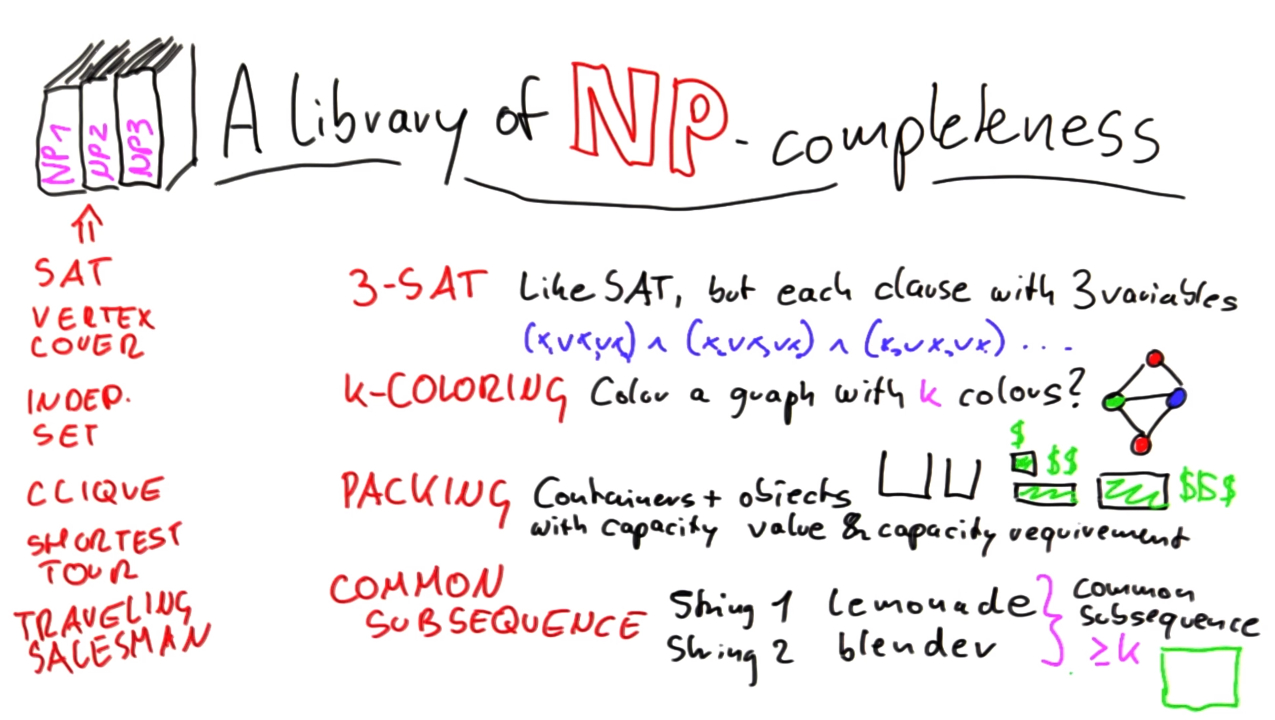
\includegraphics[width=\textwidth]{npcomplete.jpg}\\ 
Please spend as much time on this problem as the previous. It's important to make the connection 
of these concepts for yourself.
\newpage
\noindent F. Given an undirected graph $G$, design an algorithm to list the vertices in each connected component of $G$ separately.
\newpage
\noindent 10. Give an $O(V)$ time algorithm to determine whether a connected undirected graph contains a cycle.
\newpage 
\noindent The vertex cover problem states given $G$ $=$ $(V,E)$, we 
want to know the minimum size of the vertex cover $C$ $\subseteq$ $V$, where $C$ is a vertex cover if every 
edge $e$ $=$ $(u,v)\in E$ has at least of of it's endpoints $u$ or $v$ $\in C$.
(The problem generally is NP-Complete but given certain simple graphs the problem is not nearly as hard to solve).\\\\
11. Suppose that $G$ is a tree. Give a polynomial time algorithm to find the
minimum vertex cover. (Hint: Consider being greedy — and remember that you
can choose the optimal solution you like.)
\newpage
\noindent \centerline{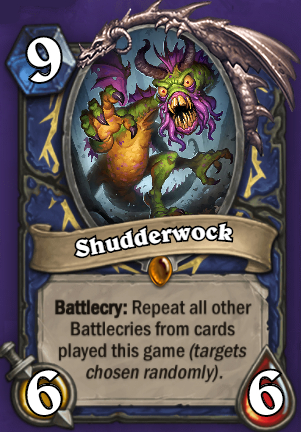
\includegraphics[scale = 2]{shudderwock.jpg}}
Blizzard has a popular card game called Hearthstone. In it 
there exists a game mechanic called battlecry, which whenever a card is played,
 that battlecry is put into effect. In the witchwood expansion they added a card called
 ``Shudderwock" which due to it's high cost can only be played towards the end of a game. It's battlecry 
 introduces recursion to Hearthstone when paired with certain cards. Recursion often breaks card games because it 
 allows for players to spam their opponents leading to unfun scenarios.\\\\
 If you have a card which includes the battlecry: plays the previous battlecry twice, you can begin 
 calling multiple Shudderwocks which will spawn infinitely. Let's try to see if we can help them out!(problems 12-14)\\\\
12. Express the mechanic that leads to recursion in a card game formally with input and output states as a \textit{decision problem}.
\newpage
\noindent 13. Show this problem is in NP by giving a verification algorithm for this problem and proving that algorithm is correct. \\\\\\\\\\\\\\\\\\\\\\\\\\\\\\\\
14. The Hamiltonian cycle problem is already known to be NP-complete. We can show that the recursion problem in card games is NP complete by reducing the Hamiltonian cycle problem to the card game recursion problem. Do so by first giving a reduction of Hamiltonian cycle problem to card game recursion problem. The reduction takes input to Hamiltonian cycle problem and converts it into input to the card game recursion problem. Then prove your reduction is correct.

\newpage
\noindent 15. What is the key difference in the problem of change making from that of prime factorization? That is to say,
what is different about these two problems that restricts us from reducing change making to prime factorization? Why is one problem 
\textit{hard} while the other is said to be \textit{easy}? 
\newpage
\noindent 16. Given an even number of coins in a row of arbitrary denominations, two players take turns taking a coin from either end. 
Winner is who gets the most cash. Player 1 goes first. 
Is there a strategy for player 1 that guarantees at least as much money as player 2?
\end{document}